\documentclass[a4paper,12pt]{amsart}
\usepackage{amssymb}
\usepackage{tikz}
\usetikzlibrary{arrows}
\usepackage{xcolor}
\usepackage{tikz,pgf}
\usetikzlibrary{patterns,spy,angles}
\usepackage{tikz-cd}

\newcommand{\io}{\mathtt{i}}

\begin{document}

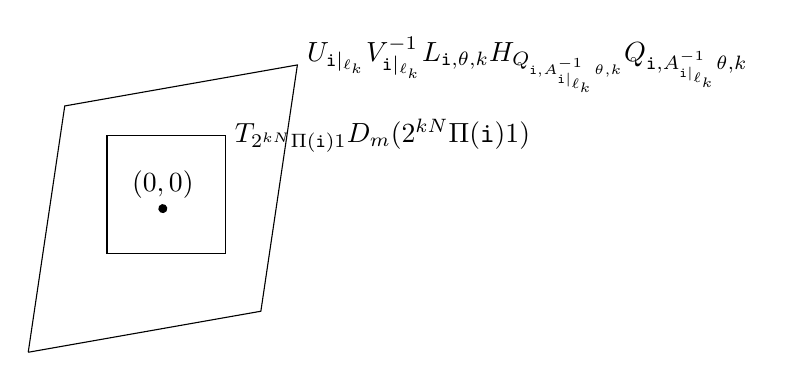
\begin{tikzpicture}
    \draw[rotate=10] (0,0) -- (3,0) -- (4,3) node[right]{$U_{\io|_{\ell_k}} V_{\io|_{\ell_k}}^{-1} L_{\io,\theta,k} H_{Q_{\io,A_{\io|_{\ell_k}}^{-1}\theta, k}}Q_{\io, A_{\io|_{\ell_k}}^{-1}\theta, k}$} -- (1,3) -- (0,0);
    \draw (1,1.25) rectangle (2.5,2.75) node[right]{$ T_{2^{kN}\Pi(\io)\mod 1}D_m(2^{kN} \Pi(\io)\mod 1)$};
    \draw[rotate=10, fill=black] (2, 1.5) node[above]{$(0,0)$} circle (0.05cm);
\end{tikzpicture}

\end{document}